% ============================================================================
% Structure-Preserving Dynamical Low-Rank Approximation of the
% Incompressible Navier--Stokes Equations in High-Reynolds-Number Turbulence
%
% Venue-neutral scaffold. The venue is not yet decided (reviewer decision D5:
% working direction is a scientific-computing / ML-adjacent venue). To target
% a specific venue, replace \documentclass and adjust the preamble to the
% venue's template; the section structure is intended to survive that swap.
% ============================================================================
% TODO(venue): swap documentclass for the venue template, e.g.
%   \documentclass[review]{icml2027}   or   \documentclass{neurips_2027}
%   or a journal class (SISC / JCP).
\documentclass[11pt]{article}

\usepackage[margin=1in]{geometry}
\usepackage{amsmath,amssymb,amsthm}
\usepackage{graphicx}
\usepackage{booktabs}
\usepackage{hyperref}
\usepackage{xcolor}

\newtheorem{proposition}{Proposition}
\newtheorem{lemma}{Lemma}
\newtheorem{remark}{Remark}

% Notation shortcuts used across sections
\newcommand{\dd}{\,\mathrm{d}}
\newcommand{\R}{\mathbb{R}}
\newcommand{\T}{\mathbb{T}}
\newcommand{\norm}[1]{\left\lVert #1 \right\rVert}
\newcommand{\inner}[2]{\left\langle #1, #2 \right\rangle}
\newcommand{\grad}{\nabla}
\newcommand{\ddt}{\partial_t}
\newcommand{\dlra}{SP-DLRA}

% Placeholder convention: [PENDING-<owner>: detail] marks every value or
% statement that must be filled from verified project data before submission.
% % [PENDING-CODER]      -> numbers / figures / scheme confirmations
% % [PENDING-THEORETICAL-RESEARCH] -> forcing-aware invariant, rank theory
% % [FLAG-<owner>]        -> open question for another agent (see README.md)

\title{Structure-Preserving Dynamical Low-Rank Approximation of the
Incompressible Navier--Stokes Equations in High-Reynolds-Number Turbulence}

\author{
  [Authors to be added]\\
  [Affiliations to be added]
}

\date{}

\begin{document}

\maketitle

\begin{abstract}
Approximating the state to cut the cost of a Navier--Stokes solve raises a
question usually asked backwards: not how accurately a reduced model tracks a
trajectory, but when a reduced trajectory is worth having. In forced
two-dimensional stream-function flow, a structure-preserving projected integrator
treats the viscous part exactly and the nonlinear part by midpoint.
Against a static subspace of equal rank, we measure the horizon at which it
is more accurate --- $t^\ast = 0.649$ at rank $16$ and
$1.482$ at rank $32$ --- and find it reflects how the subspace is built,
not its dimension: from rank $16$ the static subspace stops improving altogether, with
ranks $16$, $32$ and $43$ identical at every horizon and both Reynolds
numbers, while ranks $2$, $4$ and $8$ differ by up to $85\%$. A fixed basis propagated
through the nonlinearity overflows at ranks $32$ and $42$, reaching $10^{278}$; every structure-preserving variant holds roundoff divergence; under grid
refinement the reduced error falls by a factor $2.2$ while the static baseline's
grows by three orders of magnitude. The evidence is narrow: one
forcing, horizons of order unity, a rank criterion we report but do not
extrapolate, and a per-step cost $2.1$--$2.7\times$ the full grid with no memory
saving. We identify no end-to-end speedup, and say so.
\end{abstract}


% Introduction

\section{Introduction}
\label{sec:intro}

The incompressible Navier--Stokes (NS) equations govern fluid motion across
scales, from geophysical flows to industrial aerodynamics. At high Reynolds
numbers their dynamics are turbulent: energy cascades across a broad range of
scales and the flow field must be resolved on a fine grid for every time step
of a long simulation \cite{batchelor1969,orszag1971}. Even in two
dimensions, where the problem is comparatively tractable, the cost of a
full-resolution simulation grows steeply with the Reynolds number
\cite{vinograd2026}. Reduced representations offer a way out when the
\emph{dynamically active} degrees of freedom --- the directions in which the
solution actually moves --- are few.

Two families of methods are central here. \emph{Proper orthogonal
decomposition} (POD) constructs a fixed orthonormal basis of dominant
spatial modes from data and truncates the dynamics onto it
\cite{sirovich1987,lumley1967}. POD-based reduced order models (ROMs) for the
incompressible NS equations are mature: POD--Galerkin projections
\cite{loorenzi2016,hijazi2020,girfoglio2022pod}, stabilized and
hyper-reduced variants \cite{siena2024,star2021,klein2023}, and
closure-based extensions \cite{prakash2024}. Their limitation is
staticity: the basis is built offline on a training set and cannot follow the
dynamics when the relevant modes change over time --- exactly what happens in
sustained turbulent forcing, where new structures continually appear
\cite{vinograd2026}.

\emph{Dynamical low-rank approximation} (DLRA) makes the representation
dynamic: the solution is kept in factored form $X(t) \approx U(t)\,S(t)\,V(t)^\top$
with a small rank $r(t)$, and the factors are advanced in time so that the
basis \emph{follows} the dynamics \cite{koch2019dlra}. Projector-splitting
and structure-preserving variants integrate the linear part of the dynamics
exactly, which makes DLRA both accurate and efficient for stiff problems
\cite{einkemmer2023,ceruti2024,einkemmer2024review}. Rank adaptation ---
growing the rank when the residual demands it --- is standard via incremental
singular value decomposition \cite{haasdonk2012}.

The incompressible constraint changes the picture. The divergence-free
condition $\nabla \cdot u = 0$ is a hard geometric constraint of the
dynamics: any reduced method that violates it, even slightly, can corrupt
long-time invariants such as the energy balance. Existing low-rank approaches
to NS-type problems fall short in different ways. POD--Galerkin ROMs enforce
divergence only in a variational sense of the underlying discretization and
use static bases \cite{loorenzi2016,hijazi2020,star2021}. Reduced models in
the stream function--vorticity formulation are divergence-free by
construction, but to date they are offline or hybrid and have been validated
only at low to moderate Reynolds number: the POD--Galerkin model of Girfoglio
et al.~\cite{girfoglio2022pod} is built offline on a fixed training set, and
the hybrid model of Zhang et al.~\cite{zhang2024} combines
neural-network-corrected POD modes with DMD-based sampling for a parametric
problem; neither is rank-adaptive. Low-rank solvers for NS with uncertain or
stochastic parameters target a different problem and are not adaptive in time
\cite{lee2017,elman2019low,olshanskii2024}. The one dynamical low-rank method
applied to the incompressible equations that we are aware of is the
dynamically orthogonal (DO) approximation of Musharbash and
Nobile~\cite{musharbash2018} for stochastic problems with random boundary
conditions, with an error analysis by Musharbash, Nobile and
Zhou~\cite{musharbash2015}; it is a first cousin of DLRA --- a method of the
same family of tangent-projected, factorisation-based, on-the-fly low-rank
reduction --- but it uses a different projection and targets a stochastic
problem, not the deterministic turbulent dynamics studied here. A low-rank
projector-splitting method for weakly compressible
flow~\cite{einkemmer2018} recovers the incompressible limit as a low-rank
regime of a weakly compressible system, where the divergence constraint is not
enforced.

\paragraph{This work.}
We develop a \emph{structure-preserving} dynamical low-rank method for the
\emph{incompressible} NS equations in which (i) the viscous part is
integrated exactly, preserving the rank; (ii) the velocity is represented by a
stream function, so divergence-freeness holds identically in exact
arithmetic, with a measured residual no larger than $1.1\times10^{-13}$ for
the reduced integrator and the full-grid reference, and no larger than
$1.1\times10^{-11}$ over every method we ran --- seven orders of magnitude
below the reduced solver's own error; and (iii) the subspace is refitted as
the dynamics develop, which we show is necessary: a fixed basis propagated
through the nonlinearity overflows at ranks $32$ and $42$ where the refitted
one does not. We validate the method on forced two-dimensional flow at
Reynolds numbers $100$, $1000$ and $5000$ against a full-grid spectral
reference and a static POD baseline, and we benchmark cost honestly: the
reduced integrator is $2.1$--$2.7\times$ the full-grid step in every regime
we measured, with no compensating memory benefit.

% [FLAG-D4 / REVIEWER: Short form of the BINDING R5d claim wording (see
% state/reviewer/reviews/2026-09-25-R5d-prior-art-map-and-final-claim.md,
% Section 2); the full form is stated in Section~\ref{sec:positioning}.
% GATED on D10-V6 implemented + V1/V2/V5/V7 closed before submission; the
% final sentence describes the validation target, not achieved results.
% Barred: "no DLRA NS solver exists" (refuted by musharbash2018); "first
% exactly divergence-free NS solver" (refuted by girfoglio2022pod and the
% classical stream-function formulation); any gap phrased as a failure to
% preserve divergence-freeness; "first structure-preserving low-rank for
% conservative PDEs" (refuted by RAIL, DOI 10.1137/23M1622921); "to our
% knowledge" on arXiv evidence alone. DO-NS is a "first cousin" of DLRA,
% never a competitor. CHECKLIST 2.1's "DLRA (Osepko et al.)" could not be
% located on arXiv (0 author hits, 2026-09-25) - flagged below and in
% README.md.]
% [FLAG-WRITING-RESEARCH: confirm Osepko et al. citation, if it exists]
Our novelty claim is deliberately narrow and is stated in full in
Section~\ref{sec:positioning}.  In short: for the incompressible
Navier--Stokes equations, the existing dynamical low-rank work we are aware
of is the dynamically orthogonal approximation of Musharbash and
Nobile~\cite{musharbash2018} for stochastic problems with random boundary
conditions, and the existing reduced models in the stream
function--vorticity formulation are offline and hybrid
\cite{girfoglio2022pod,zhang2024}; we are not aware of a structure-preserving,
exactly divergence-free, factorisation-based low-rank integrator for the
deterministic incompressible Navier--Stokes equations, or of any dynamical
low-rank method for that setting validated in a resolved
high-Reynolds-number forced-turbulent regime.  We provide one: we apply the
established robust basis-update-and-Galerkin machinery to the stream
function--vorticity formulation, in which divergence-freeness holds exactly
by representation, and validate it against a full-grid spectral reference at
Reynolds numbers $\mathrm{Re} \in \{100, 1000, 5000\}$ with adaptive rank.

\paragraph{Paper organization.}
Section~\ref{sec:contributions} states our contributions.
Section~\ref{sec:related} reviews related work. Section~\ref{sec:methods}
develops the method: the stream-function formulation and energy identity
(4.1--4.2), the structure-preserving split and exact viscous lemma
(4.3), the projected nonlinear step (4.4), rank adaptation (4.5), the
invariants (4.6), and cost (4.7). Section~\ref{sec:setup} describes the
experimental setup and validation ladder; Section~\ref{sec:results} reports
results; Sections~\ref{sec:discussion}--\ref{sec:limitations} discuss
interpretation and limitations; Section~\ref{sec:conclusion} concludes.

% Contributions

\section{Contributions}
\label{sec:contributions}

Our contributions are:

\begin{enumerate}
  \item \textbf{A structure-preserving DLRA scheme for the 2D incompressible
  NS equations in stream-function form.} The viscous part of the dynamics is
  integrated \emph{exactly} along a separable exponential flow that preserves
  the low-rank ansatz (Section~\ref{sec:methods}, Proposition~\ref{prop:viscous});
  the velocity is represented through a stream function, so the discrete
  velocity is exactly divergence-free at every time step and for every rank,
  to machine precision (Invariant I1, Section~\ref{sec:invariants}).

  \item \textbf{A second-order projected nonlinear step with online rank
  adaptation.} The nonlinear (advective plus forcing) part is advanced by a
  midpoint step on the projected dynamics, and the rank is grown online by
  incremental singular value decomposition when a residual-based error
  indicator exceeds tolerance (Section~\ref{sec:rank-adaptation}).

  \item \textbf{Validation on forced high-Reynolds-number turbulent dynamics.}
  We run the method on forced 2D turbulence at Reynolds numbers
  $100$, $1000$, and $5000$ (Section~\ref{sec:setup}), verify the invariants
  (I1--I4), and compare against (a) a full-grid spectral reference for
  accuracy and (b) a static POD baseline for the cost of staticity:
  fixed-basis POD cannot follow the rank growth that sustained forcing
  induces (Section~\ref{sec:results}).

  \item \textbf{Honest benchmarking.} We report per-step and total cost
  against the full-grid spectral reference and the POD baseline, including
  the regimes in which SP-DLRA is \emph{slower}
  (Section~\ref{sec:cost}, Figure~\ref{fig:cost}).
\end{enumerate}

% [PENDING-CODER: contribution 3 and 4 become quantitative once results land;
% keep the qualitative framing until then.]

% Related work

\section{Related Work}
\label{sec:related}

We organize the related work into three threads: dynamical low-rank methods
and projector splitting; reduced order models for the incompressible NS
equations; and low-rank approaches that are closest in setting to ours.

\subsection{Dynamical low-rank approximation and projector splitting}
\label{sec:related:dlra}

DLRA approximates a high-dimensional trajectory by a low-rank matrix whose
factors evolve in time; the original formulation is due to Koch and
Lubich~\cite{koch2007}, with early numerical experiments on reaction--diffusion
PDEs by Nonnenmacher and Lubich~\cite{nonnenmacher2008}. The key practical idea
for stiff dynamics is
the \emph{projector split}: integrate the linear part exactly with the frozen
factors, then update the factors for the nonlinear part
\cite{lubich2014}. The most recent work on the split itself is the augmented
backward-corrected projector-splitting integrator of Kusch, Schotthöfer and
Walter~\cite{kusch2026augmented}, which targets the training of dynamical
low-rank models for data assimilation rather than the time integration of a
conservative PDE, and so addresses a different question from the one we pose
here; we cite it as the closest modern projector-splitting method. Rank
adaptation via incremental SVD (the row-action technique) makes the rank grow
only when needed \cite{haasdonk2012}.
Stability of robust projector-splitting schemes has been analyzed for
hyperbolic problems \cite{kusch2023stability}; robustness and conservation
properties have been established for kinetic equations \cite{einkemmer2023},
and second-order variants such as the midpoint-based low-rank BUG integrator
improve accuracy at comparable cost \cite{ceruti2024}. Reduced augmentation
implicit low-rank (RAIL) integrators extend the machinery to advection--
diffusion and Fokker--Planck models \cite{rail2025}, and a macro-micro
decomposition for consistent, conservative model order reduction of hyperbolic
shallow-water moment equations has been studied against both DLRA and
POD--Galerkin \cite{koellermeier2024}. A recent review places these methods in
the context of time-dependent kinetic simulation \cite{einkemmer2024review}.
The structure-preserving (SP) variant used here --- exploiting that the linear
operator's exponential acts on the two factor families independently --- has
recently been applied to stochastic Vlasov--Poisson dynamics \cite{cui2026}
and to parametric elastic guided-wave propagation \cite{goutaudier2026}. None
of the DLRA works surveyed in this subsection targets the incompressible
Navier--Stokes equations or the divergence-free constraint; the closest
dynamical work in that setting is the dynamically orthogonal approximation,
discussed in Section~\ref{sec:related:ns}.

\subsection{Reduced order models for the incompressible NS equations}
\label{sec:related:rom}

The POD--Galerkin literature is extensive. Classical POD--Galerkin models for
finite-volume discretizations \cite{loorenzi2016} and data-driven
POD--Galerkin models for turbulent flows \cite{hijazi2020} enforce
divergence in the variational sense of the underlying discretization;
stabilized POD ROMs for convection-dominated flows \cite{siena2024},
collocated `discretize-then-project' models \cite{star2021}, and
hyper-reduced / temporally localized models \cite{klein2023} address
stability and efficiency. Closure-based approaches
\cite{prakash2024} and domain-decomposition ROMs \cite{prusak2023} target
parametric and large-scale settings, and data-driven parametrizations combine
POD with neural components \cite{kim2023,kochkov2021}. The closest in formulation are the reduced models in the stream
function--vorticity formulation, in which the reduced velocity is
divergence-free by construction: the POD--Galerkin model of Girfoglio
et al.~\cite{girfoglio2022pod} is built offline on a fixed training set and
validated on canonical flows at low to moderate Reynolds number, while the
hybrid model of Zhang et al.~\cite{zhang2024} combines neural-network-
corrected POD modes with DMD-based sampling for a parametric problem. Neither
is rank-adaptive, and neither has been validated in a resolved
high-Reynolds-number turbulent regime.

\subsection{Dynamical and low-rank methods for the incompressible Navier--Stokes equations}
\label{sec:related:ns}

The dynamical low-rank work we are aware of for the incompressible NS
equations is the dual dynamically orthogonal (DO) approximation of Musharbash
and Nobile~\cite{musharbash2018} for stochastic problems with random boundary
conditions, with an error analysis by Musharbash, Nobile and
Zhou~\cite{musharbash2015}. DO-NS is a first cousin of DLRA --- a method of
the same family of tangent-projected, factorisation-based, on-the-fly
low-rank reduction --- but a different method: it uses a different projection
and targets a stochastic problem with random boundary data, not the
deterministic forced-turbulent dynamics studied here. It is not a competitor
in this setting; the gap between DO-NS and the present work is stated in
Section~\ref{sec:positioning}. Other low-rank methods for NS-type problems
are further from the present setting: solvers for the NS equations with
uncertain viscosity \cite{lee2017} and for the stochastic unsteady problem
\cite{elman2019low} exploit low-rank structure in the \emph{parameter or
random} direction of steady or mildly unsteady problems and are not adaptive
in time, and ROMs that approximate branches of NS solutions
\cite{olshanskii2024} target bifurcation structure rather than turbulent
dynamics. A low-rank projector-splitting method for weakly compressible
flow~\cite{einkemmer2018} recovers the incompressible limit as a low-rank
regime of a weakly compressible system, where the divergence constraint is
not enforced.

\subsection{Positioning and comparison}
\label{sec:positioning}

Table~\ref{tab:related} compares the closest prior work along the axes
that matter for our claim: whether the method is dynamical (online rank
adaptation), whether it is exactly divergence-free by construction, and
whether it has been validated on high-Reynolds-number turbulent dynamics.

\begin{table}[h]
\centering
\small
\begin{tabular}{@{}lccc@{}}
\toprule
Method & Dynamical & Exactly & High-Re \\
       & (rank) & divergence-free & turbulence \\
\midrule
POD--Galerkin, stream-function--vorticity \cite{girfoglio2022pod} & $\times$ & $\checkmark$ & $\times$ \\
Data-driven POD--Galerkin \cite{hijazi2020} & $\times$ & variational & partial \\
POD--Galerkin, finite volume \cite{loorenzi2016} & $\times$ & variational & partial (RANS) \\
Stabilized POD ROM \cite{siena2024} & $\times$ & $\times$ & $\times$ \\
Collocated DTP POD--Galerkin \cite{star2021} & $\times$ & $\times$ & $\times$ \\
Hyper-reduction + temporal localization \cite{klein2023} & partial & $\times$ & $\times$ \\
Closure-based projection ROM \cite{prakash2024} & $\times$ & $\times$ & $\times$ \\
Domain-decomposition POD--Galerkin \cite{prusak2023} & $\times$ & $\times$ & $\times$ \\
POD + neural parametrization \cite{kim2023,kochkov2021} & $\times$ & $\times$ & $\times$ \\
Low-rank NS, uncertain viscosity \cite{lee2017} & $\times$ & $\times$ & $\times$ \\
Low-rank stochastic unsteady NS \cite{elman2019low} & $\times$ & $\times$ & $\times$ \\
ROM of solution branches \cite{olshanskii2024} & $\times$ & $\times$ & $\times$ \\
Low-rank weakly compressible flow \cite{einkemmer2018} & $\checkmark$ & $\times$ & $\times$ \\
Dynamically orthogonal NS (stochastic) \cite{musharbash2018} & $\checkmark$ & n/a & $\times$ \\
Hybrid POD/DMD ROM, stream--vorticity \cite{zhang2024} & $\times$ & $\checkmark$ & $\times$ \\
RAIL integrators (adv.--diff., Fokker--Planck) \cite{rail2025} & $\checkmark$ & n/a & n/a \\
Robust/conservative DLRA (kinetic) \cite{einkemmer2023} & $\checkmark$ & n/a & n/a \\
Low-rank midpoint BUG integrator (kinetic) \cite{ceruti2024} & $\checkmark$ & n/a & n/a \\
SP-DLRA, stochastic Vlasov--Poisson \cite{cui2026} & $\checkmark$ & n/a & n/a \\
SP-DLRA, elastic guided waves \cite{goutaudier2026} & $\checkmark$ & n/a & n/a \\
Review (kinetic low-rank methods) \cite{einkemmer2024review} & review & n/a & n/a \\
\midrule
% [FLAG-D4 / REVIEWER: High-Re cell is "target", not a checkmark, per D10:
% the claim is gated on D10-V6 implemented + V1/V2/V5/V7 closed. Do not
% change to $checkmark until the validation ladder is complete.]
\textbf{This work (SP-DLRA for incompressible NS)} & $\checkmark$ & $\checkmark$ & target \\
\bottomrule
\end{tabular}
\caption{Comparison of the closest prior work. ``Dynamical'': online rank
adaptation; ``Exactly divergence-free'': the discrete velocity satisfies
$\nabla\cdot u = 0$ to machine precision by construction (not only in a
variational sense); ``High-Re turbulence'': validated on forced,
high-Reynolds-number turbulent dynamics. Entries marked ``partial'',
``variational'', ``n/a'', or ``target'' are qualified in the text; for the
dynamically orthogonal NS method the by-construction divergence-freeness
column does not apply (no stream-function representation) and is not
evaluated here; ``target'' marks the validation regime of the present work
(Section~\ref{sec:setup}), pending the validation ladder.}
\label{tab:related}
\end{table}

% [FLAG-WRITING-RESEARCH + REVIEWER: CHECKLIST 2.1 requires covering
% "DLRA (Osepko et al.)". No author "Osepko" was found on arXiv (0 hits,
% 2026-09-25) and a full-text search for "dynamical low-rank" with
% incompressible Navier--Stokes also returned 0 results. Not cited: policy is
% that nothing unverifiable goes in the bibliography. Awaiting the exact
% citation from reviewer / writing-research; the row will be added here once
% identified.]
% [FLAG-D4 / REVIEWER: BINDING R5d claim wording (state/reviewer/reviews/
% 2026-09-25-R5d-prior-art-map-and-final-claim.md, Section 2), full form;
% the short form appears in Section~\ref{sec:intro}. GATED on D10-V6
% implemented + V1/V2/V5/V7 closed before submission; the final sentence
% describes the validation target, not achieved results. Barred: "no DLRA NS
% solver exists" (refuted by musharbash2018); "first exactly divergence-free
% NS solver" (refuted by girfoglio2022pod and the classical
% stream-function formulation); any gap phrased as a failure to preserve
% divergence-freeness; "first structure-preserving low-rank for conservative
% PDEs" (refuted by RAIL, DOI 10.1137/23M1622921); "to our knowledge" on
% arXiv evidence alone. DO-NS is a "first cousin" of DLRA, never a
% competitor.]
Structure-preserving dynamical low-rank approximation is well established for
Hamiltonian, kinetic, Vlasov--Poisson and wave equations, and robust low-rank
integrators for conservative PDEs (advection--diffusion, hyperbolic moment
systems) are established as well
\cite{koch2007,lubich2014,kusch2023stability,einkemmer2023,ceruti2024,
rail2025,koellermeier2024,cui2026,goutaudier2026,einkemmer2024review}. For the incompressible Navier--Stokes equations, the
existing dynamical low-rank work we are aware of is the dynamically
orthogonal approximation of Musharbash and Nobile~\cite{musharbash2018} for
stochastic problems with random boundary conditions, and the existing
reduced models in the stream function--vorticity formulation are offline and
hybrid \cite{girfoglio2022pod,zhang2024}.

We are not aware of a structure-preserving, exactly divergence-free,
factorisation-based low-rank integrator for the deterministic incompressible
Navier--Stokes equations, or of any dynamical low-rank method for that
setting validated in a resolved high-Reynolds-number forced-turbulent regime.

We provide one: we apply the established robust basis-update-and-Galerkin
machinery to the stream function--vorticity formulation, in which
divergence-freeness holds exactly by representation, and validate it against
a full-grid spectral reference at Reynolds numbers $\mathrm{Re} \in \{100,
1000, 5000\}$ with adaptive rank.

% Methods

\section{Method}
\label{sec:methods}

\subsection{Problem setup and notation}
\label{sec:problem}

We consider the two-dimensional incompressible Navier--Stokes equations on the
periodic torus $\T^2 = [0,2\pi]^2$, the classical periodic setting of
Leray~\cite{leray1934}:
\begin{equation}
  \partial_t u + (u\cdot\grad)u = \nu\,\Delta u + f,
  \qquad \grad\cdot u = 0,
  \label{eq:ns}
\end{equation}
where $u = (u_1,u_2): \T^2 \to \R^2$ is the velocity, $\nu > 0$ the kinematic
viscosity, and $f$ an externally prescribed body force. Throughout we use
single-mode Kolmogorov forcing
\begin{equation}
  f = F \sin y \; e_x, \qquad F > 0,
  \label{eq:forcing}
\end{equation}
whose curl is $\grad \times f = -F\cos y$. The Reynolds number is defined as
$\mathrm{Re} = 2U/\nu$, with $U$ the Kolmogorov base speed and $L = 2\pi$ the
domain size; equivalently $\mathrm{Re} = U/(\nu k)$ at the fundamental
$k = \pi/L = 1/2$. The pairing of $F$ and $\nu$ for each Reynolds number is
given per run in Table~\ref{tab:forced-params} (Section~\ref{sec:forced}).

Since the domain is periodic, the force has zero mean, and $\grad \cdot u = 0$,
there exists a zero-mean stream function $\psi$ with
\begin{equation}
  u = (\partial_y \psi, -\partial_x \psi),
  \qquad \omega := \grad \times u = -\Delta \psi,
  \label{eq:stream}
\end{equation}
where $\omega$ is the vorticity. This sign convention is used throughout.
Substituting \eqref{eq:stream} into \eqref{eq:ns} and taking the curl yields
the stream-function formulation
\begin{equation}
  \partial_t \psi
  = \nu\,\Delta \psi + \Delta^{-1} J(\psi, \Delta \psi) - F \cos y,
  \qquad
  J(\psi, \varphi) := \partial_x \psi\, \partial_y \varphi
                      - \partial_y \psi\, \partial_x \varphi,
  \label{eq:stream-ns}
\end{equation}
where $\Delta^{-1}$ is the exact Fourier inverse on the zero-mean subspace.
The velocity is recovered from $\psi$ via \eqref{eq:stream} at every step, so
the discrete velocity is divergence-free by construction (Invariant I1,
Section~\ref{sec:invariants}).

All fields are represented on an $N \times N$ tensor-product Fourier
collocation grid ($n = N^2$ grid points); $\Delta$ and $\Delta^{-1}$ are the
spectral operators, and all $L^2$ norms below are the discrete
ell-two norms, which are spectrally equivalent on the collocation grid.
Identifying a field with its $N \times N$ matrix of values (rows indexed by
$x$, columns by $y$), the Laplacian separates as
\begin{equation}
  \Delta = D_x \otimes I + I \otimes D_y,
  \qquad D_x := -\partial_{xx}, \quad D_y := -\partial_{yy},
  \label{eq:lap-sep}
\end{equation}
with $[D_x \otimes I, \; I \otimes D_y] = 0$. This separation is the
structural fact exploited by the scheme.

\subsection{Energy identity}
\label{sec:energy}

Let $E(t) = \tfrac{1}{2}\norm{u}_2^2 = \tfrac{1}{2}\norm{\grad\psi}_2^2$ be the
kinetic energy. Taking the $L^2$ inner product of \eqref{eq:stream-ns} with
$\Delta \psi$ (equivalently, pairing the vorticity equation with
$\Delta^{-1}\omega$) gives
\begin{equation}
  \frac{\dd E}{\dd t}
  = \underbrace{\inner{u}{f}}_{P_{\mathrm{in}}(t)}
  \;-\;
  \underbrace{\nu\, \norm{\Delta \psi}_2^2}_{P_{\mathrm{diss}}(t)},
  \label{eq:energy}
\end{equation}
where the advective term is exactly energy-neutral (a standard identity for
periodic, divergence-free flows; see Temam~\cite{temam1977}) and the forcing
power is
\begin{equation}
  P_{\mathrm{in}}(t)
  = \inner{u}{f}
  = F\,\inner{\psi_y}{\sin y}
  = -F\,\inner{\psi}{\cos y},
  \label{eq:pin}
\end{equation}
with the last equality by integration by parts on the torus. The forced
system possesses the Kolmogorov equilibrium
\begin{equation}
  \psi_K = -\frac{F}{\nu}\cos y,
  \qquad
  u_K = \frac{F}{\nu}\sin y \; e_x,
  \label{eq:kolmogorov}
\end{equation}
at which \eqref{eq:energy} gives $P_{\mathrm{in}} = P_{\mathrm{diss}}
= 2\pi^2 F^2/\nu$. That equilibrium is an exact solution of the discretised
equations for any $(F,\nu)$: the diffusion and forcing terms cancel, and the
advection of $\omega_K$ vanishes identically. It is not, however, the state the
runs are started from --- Section~\ref{sec:setup} records how far below it they
begin.
% [RESOLVED from solvers/ns_psi.py: the 2/3 mask is applied to the field-level
% nonlinear and advection terms and not to the viscous semigroup;
% energy_terms() computes the advection term explicitly rather than assuming it
% vanishes, with zeta = -A cos y so that -<psi,zeta> = +A<psi,cos y> = P_in.]

Two consequences matter for the validation design. First, under forcing the
kinetic energy is \emph{not} monotone: $E(t)$ relaxes toward the forced
statistical regime with $P_{\mathrm{in}}(t) \approx P_{\mathrm{diss}}(t)$ on
average, and the relevant forcing-aware invariant is developed by the theory
work (Invariant I2, Section~\ref{sec:invariants};
% [PENDING-THEORETICAL-RESEARCH: forcing-aware invariant, docs/theory/
% stability-error.md]).
Second, the unforced limit $F = 0$ reduces \eqref{eq:energy} to
$\dd E/\dd t = -P_{\mathrm{diss}} \le 0$, so the laminar Taylor--Green decay
test must exhibit monotone non-increasing $E(t)$ (Section~\ref{sec:setup}).

\subsection{SP-DLRA ansatz and the exact viscous step}
\label{sec:spd}

We seek $\psi$ in the rank-$r$ ansatz
\begin{equation}
  \Psi := \psi \approx U S V^{\top},
  \qquad U, V \in \R^{N \times r}, \quad S \in \R^{r \times r},
  \label{eq:ansatz}
\end{equation}
with orthonormal columns $U^{\top}U = V^{\top}V = I_r$ and $S \succeq 0$
symmetric ($\Psi = USV^{\top}$ is its thin SVD; $r \ll N$). The
\emph{structure-preserving} property we exploit is that the viscous flow
preserves this ansatz \emph{exactly}.

\begin{proposition}[Exact, rank-preserving viscous step]
\label{prop:viscous}
Let $\Psi = USV^{\top}$ have rank $r$ with full-rank factors, and let
$\Delta = D_x \otimes I + I \otimes D_y$ as in \eqref{eq:lap-sep}. Then for
all $t \ge 0$,
\begin{equation}
  e^{\nu t \Delta}\, \Psi
  =
  \left(e^{\nu t D_x} U\right)\, S \,
  \left(e^{\nu t D_y} V\right)^{\top}.
  \label{eq:viscous-exact}
\end{equation}
In particular the viscous flow preserves the rank-$r$ ansatz exactly: the
evolved factors are $\hat U = e^{\nu t D_x} U$ and
$\hat V = e^{\nu t D_y} V$, and the singular values $S$ are unchanged.
\end{proposition}

\begin{proof}
$D_x \otimes I$ and $I \otimes D_y$ commute, so
$e^{\nu t \Delta} = e^{\nu t (D_x \otimes I)}\, e^{\nu t (I \otimes D_y)}$.
For any matrix $X$, $e^{\nu t (D_x \otimes I)} X = (e^{\nu t D_x} X)$, since
$D_x \otimes I$ applies $D_x$ row-wise; and, since $D_y$ is symmetric,
$X\, e^{\nu t (I \otimes D_y)} = X\, (e^{\nu t D_y})^{\top}$, since
$I \otimes D_y$ applies $D_y$ column-wise. Applying both to
$\Psi = USV^{\top}$ gives \eqref{eq:viscous-exact}.
\end{proof}

\begin{remark}[Cost of the viscous step]
$e^{\nu t D_x} U$ is computed column-wise by one-dimensional FFTs in the $x$
direction at cost $O(r N \log N) = O(r n \log n)$ (likewise for $V$). The full
viscous step is therefore $O(r n \log n)$, exact, and requires no SVD. This
is the cost of the viscous stage. The rank rule is separate: as implemented,
it factorizes the whole field at four stage boundaries per step, so the
per-step cost is $\Theta(N^3)$ and \textbf{independent of $r$} --- $r=2$ and
$r=64$ cost the same, because the truncated reconstruction changes only which
columns of an already-computed factorization are used --- measured, the ratio of
the $r=64$ to the $r=2$ full-step cost is $1.13$ at $N=64$ and within $5\%$ at
the two finer grids, against per-configuration timing spreads of order $1\%$.
Per-stage rank updates would invert this; we report the implemented behaviour
rather than the asymptotic one.
\end{remark}

\begin{remark}[What is preserved]
Equation~\eqref{eq:viscous-exact} says that the viscous semigroup is
invariant under the ansatz: the approximation error of the viscous step is
\emph{zero}, not merely small. This is the sense in which the scheme is
structure-preserving with respect to the viscous part, in the spirit of
separable/projector-splitting low-rank methods
\cite{koch2007, einkemmer2023, cui2026, goutaudier2026}. The nonlinear
part is \emph{not} invariant under the ansatz and is handled by a projected
step (Section~\ref{sec:proj-step}).
\end{remark}

\subsection{The projected nonlinear step}
\label{sec:proj-step}

Let $\Psi^n = USV^{\top}$ be the rank-$r$ approximation at time $t_n$ and let
$\Delta t$ be the time step. One SP-DLRA step is:

\begin{enumerate}
  \item \textbf{Exact viscous half-step (midpoint state).}
  \begin{equation}
    \Psi_m := e^{\nu \Delta t\, \Delta / 2}\, \Psi^n
    = \hat U S \hat V^{\top},
    \qquad
    \hat U := e^{\nu \Delta t D_x/2}\, U,
    \quad
    \hat V := e^{\nu \Delta t D_y/2}\, V,
    \label{eq:midpoint}
  \end{equation}
  by Proposition~\ref{prop:viscous} with $t = \Delta t/2$.
  \item \textbf{Nonlinear residual on the full grid.}
  \begin{equation}
    N(\Psi_m) := \Delta^{-1} J(\Psi_m, \Delta \Psi_m) - F \cos y.
    \label{eq:nonlin}
  \end{equation}
  \item \textbf{Projected midpoint update.} With the projection
  $\Pi_{\hat U, \hat V} G = \hat U (\hat U^{\top} G) \hat V^{\top}$,
  \begin{equation}
    \Psi^{n+1}
    =
    e^{\nu \Delta t\, \Delta}\, \Psi^n
    + \Delta t \; \Pi_{\hat U, \hat V}\, N(\Psi_m).
    \label{eq:step}
  \end{equation}
  Since $e^{\nu \Delta t \Delta} \Psi^n = \hat U_{\Delta t} S
  \hat V_{\Delta t}^{\top}$ (Proposition~\ref{prop:viscous}) with
  $\hat U_{\Delta t} = e^{\nu \Delta t D_x} U$,
  $\hat V_{\Delta t} = e^{\nu \Delta t D_y} V$, step \eqref{eq:step} is
  equivalently the coefficient update
  \begin{equation}
    S \leftarrow S + \Delta t\, \hat U_{\Delta t}^{\top}\,
    N(\Psi_m)\, \hat V_{\Delta t},
    \label{eq:s-update}
  \end{equation}
  on the viscously evolved factors (the Galerkin/projected integrator of
  Haasdonk and Ohlberger~\cite{haasdonk2012}).
  \item \textbf{Cleanup.} A thin SVD of $\Psi^{n+1}$ re-orthonormalizes the
  factors (rank at most $2r$ before truncation); singular values below
  tolerance are dropped (decay) and the residual indicator below may extend
  the rank (growth; Section~\ref{sec:rank-adaptation}). The SVD is of the
  \emph{whole} field, and is the dominant per-step cost of the scheme as
  implemented (Section~\ref{sec:cost}).
\end{enumerate}

The step is a \emph{projected exponential midpoint method}: the viscous part
is integrated exactly (Proposition~\ref{prop:viscous}) and the nonlinear part
is advanced by a midpoint rule on the projected dynamics, in the style of the
robust low-rank integrators of Einkemmer et al.~\cite{einkemmer2023} and
Ceruti et al.~\cite{ceruti2024}. For fixed factors the step is second order
in $\Delta t$; the projection error is the rank deficiency of the current
subspace, which the rank adaptation below is designed to control.
% [RESOLVED (D10): eq:step projects with the midpoint-evolved factors
% \hat U = e^{nu dt D_x/2} U, which the code evolves before the augmented step
% uses them, and the second-order property is asserted by
% test_reduced_path_is_second_order_in_dt and test_bug_is_second_order.]

\subsection{Adaptive rank}
\label{sec:rank-adaptation}

\paragraph{Growth (incremental SVD).}
Let $G := \Delta t\, N(\Psi_m)$ be the \emph{unprojected} nonlinear update and
$\Pi = \Pi_{\hat U, \hat V}$. We measure the component of $G$ outside the
current subspace by the residual indicator
\begin{equation}
  \eta := \frac{\norm{G - \Pi G}_F}{\norm{G}_F}.
  \label{eq:indicator}
\end{equation}
If $\eta > \eta_{\mathrm{tol}}$, the dominant direction of $G - \Pi G$ is
added to the subspace via an incremental singular value decomposition of the
augmented factors (the rank-adaptation technique of
Haasdonk and Ohlberger~\cite{haasdonk2012}), and the coefficients are
re-solved. Growth is the only \emph{active} rank change in the scheme. In the
forced runs the indicator is triggered within the first steps, the retained rank
reaches the budget, and it stays there for the rest of the run
(Section~\ref{sec:res-rank}).

\paragraph{Decay.}
At the cleanup SVD, singular values with $\sigma_i < \sigma_{\mathrm{tol}}$
(absolute) or $\sigma_i/\sigma_1 < \sigma_{\mathrm{tol}}$ (relative) are
dropped. This is a deterministic, cheap rule requiring no additional
decompositions. The implemented rule is a \emph{relative} amplitude cutoff of
$10^{-10}$ on the singular-value spectrum, tested every five steps, with the
rank requested between $2$ and the budget $2\lfloor N/3\rfloor+1$
(Section~\ref{sec:setup}); the state is carried at its own numerical rank, which
for the forced initial condition is seventeen. In the unforced Taylor--Green test
the state is a single Fourier mode, so the rule holds the rank at one from the
outset rather than spend rank on a spectrum that is not present
(Section~\ref{sec:results}).
% [RESOLVED from the run records: parameters.dlra_relative_amplitude_cutoff,
% dlra_check_every, dlra_min_rank, dlra_max_rank; the L1 run holds a fixed rank
% of one, so no tolerance is exercised there.]

\subsection{Invariants}
\label{sec:invariants}

We validate the scheme against four invariants, per reviewer decision D3:

\begin{itemize}
  \item \textbf{I1 (exact divergence-freeness).} The velocity is recovered as
  $u = (\psi_y, -\psi_x)$ from the (low-rank) stream function, so
  $\grad \cdot u = 0$ \emph{identically in exact arithmetic}. The measured
  residual never exceeds $1.1\times 10^{-11}$ over every method, rank and
  Reynolds number we ran, which is seven orders of magnitude below the reduced
  solver's own error ($\sim 10^{-4}$) and therefore cannot account for it. The
  residual is the roundoff of the discrete spectral derivative pair, and grows as
  the operators' conditioning does: $2.6\times$ from $N=64$ to $N=128$,
  consistently across methods. Section~\ref{sec:res-div} reports the measured
  band and the population it is taken over.
  \item \textbf{I2 (energy).} Unforced: $E(t)$ is monotone non-increasing
  (verified numerically in the Taylor--Green test). Forced: $E$ obeys
  \eqref{eq:energy} with $P_{\mathrm{in}} = -F\inner{\psi}{\cos y}$ and
  $P_{\mathrm{diss}} = \nu \norm{\Delta \psi}_2^2$; the forcing-aware
  invariant characterizing the statistical regime is given by the theory
  work.
  % [PENDING-THEORETICAL-RESEARCH: forcing-aware invariant and any
  % monotone/conserved quantity for the forced dynamics,
  % docs/theory/stability-error.md]
  \item \textbf{I3 (rank economy).} The adaptive rank $r(t)$ against the static
  POD count $r_{\mathrm{POD}} = 16$ --- the rank the static baselines were
  \emph{given}, not a count we measure. Their bases are fitted on the
  fluctuations of the reference run, including the initial condition, at a
  $99\%$-energy threshold. Because that rank is the requested cap and is the same
  in every run, it does not vary with the dynamics, and we therefore report the
  rank economy as a comparison against a fixed rank rather than as a measured
  saving.
  \item \textbf{I4 (turbulent fidelity).} Kinetic-energy time series,
  kinetic-energy spectrum, and dissipation statistics against the full-grid
  spectral reference.
\end{itemize}

\subsection{Cost model}
\label{sec:cost}

Per step, with $n = N^2$ grid points and rank $r$:
\begin{center}
\begin{tabular}{lll}
  \toprule
  Component & Cost & Remark \\
  \midrule
  Viscous half- and full-step (Prop.~\ref{prop:viscous}) & $O(r\, n \log n)$
    & factor-wise 1D FFT exponentials \\
  Nonlinear residual $N(\Psi_m)$ & $O(n \log n)$
    & $\Delta$, $\Delta^{-1}$ by FFT; $J$ pointwise;
    \emph{rank-independent} \\
  Projection $\Pi_{\hat U, \hat V} N(\Psi_m)$ & $O(r n)$ & \\
  Cleanup: thin SVD of the whole field, four per step & $\Theta(N^3)$ &
    \emph{rank-independent} \\
  \bottomrule
\end{tabular}
\end{center}

\paragraph{Timing protocol.} Per-step cost is the median of seven or more
repeats after a discarded warm-up, taken under two accountings --- the complete
reduced step, including the full-grid nonlinear evaluation and all projections,
and the time inside the whole-field factorizations alone --- each expressed as a
ratio against the pinned-thread full-grid reference. Configurations are
interleaved rather than run to completion one after another: on a shared node the
per-configuration median is unreliable, while the ratio between two interleaved
configurations is not. That is why we report the spreads and quote the band to one
significant figure. Two further facts belong here rather than in a footnote. The
rank is \emph{held fixed} for the timing, so the cost is measured at a fixed rank
and not under adaptation. And the benchmark state is an unforced multi-mode decay
rather than the forced initial condition, because a fixed low rank on a forced
field grows without bound and makes the factorization fail --- a property of that
configuration rather than a cost result.

The full-grid spectral reference has per-step cost $O(n \log n)$ with the same
asymptotic form. We emphasize the honest consequence: because the nonlinear
residual is evaluated on the full grid, its $O(n \log n)$ cost is
\emph{independent of the rank}, and we make no claim of per-step speedup:
SP-DLRA is measured at $2.2$--$3.5\times$ the full-grid step
(Section~\ref{sec:res-cost}, Figure~\ref{fig:cost}). Nor is there a compensating
memory benefit: peak memory is $2.3$ MiB ($N=64$) to $4.0$ MiB ($N=128$)
\emph{above} the full-grid step, because the state is a full field plus its
factors plus the factorisation workspace. We therefore identify no end-to-end
benefit in the regimes we have measured, and the case for the method rests on its
structural guarantees and its accuracy, not on efficiency. Establishing a regime
where the rank stays small over a long span would require evidence beyond the
$200$-step horizons used here, and we do not have it.
% [PENDING-CODER: the per-step cost and peak memory of SP-DLRA against the
% pinned-thread full-grid reference are measured, per grid, in
% cost_retiming.json and peak_memory.json. The static-baseline family is NOT
% timed, so there is no measured baseline cost ratio to report; this stays open
% until the coder times it.]

% Experimental setup

\section{Experimental setup}
\label{sec:setup}

The validation follows the reviewer's acceptance ladder
(CHECKLIST, items L1--L4): a laminar smoke test, forced turbulent runs at
three Reynolds numbers, a full-grid spectral reference, and a static POD
baseline.

\subsection{L1: Taylor--Green laminar decay}
\label{sec:taylor-green}

The unforced problem ($F = 0$) on $\T^2$, initialized with the Taylor--Green
stream function
\begin{equation}
  \psi_{\mathrm{TG}}(x,y,0) = A \sin x \sin y
  \qquad\Longleftrightarrow\qquad
  u_{\mathrm{TG}} = (A \sin x \cos y,\; -A \cos x \sin y),
  \label{eq:tg}
\end{equation}
with $A = 1$
% [PENDING-CODER: confirm amplitude A, viscosity nu (Re), grid N, time span,
% initial rank r_0, and rank tolerances for the L1 run.]
and viscosity $\nu$ fixed by the chosen Reynolds number
$\mathrm{Re} = 2\pi/\nu^2$
% [PENDING-CODER: confirm Re value used for the laminar decay run.]
, the flow decays monotonically: $E(t)$ is non-increasing by
\eqref{eq:energy}, and the singular values of $\psi(\cdot,\cdot,t)$ decay
rapidly. This test verifies (i) the discrete energy monotonicity (I2,
unforced), (ii) the exact divergence-free property (I1), and (iii) the
$\sigma_{\mathrm{tol}}$ decay rule of Section~\ref{sec:rank-adaptation},
which should drive the rank $3 \to 2 \to 1$ as the vortex dissipates
(Figure~\ref{fig:tg}).

\subsection{L2: forced turbulent runs}
\label{sec:forced}

The main experiments are forced Kolmogorov-flow runs with
$f = F\sin y\, e_x$ at
\begin{equation}
  \mathrm{Re} \in \{100,\; 1000,\; 5000\},
  \qquad \mathrm{Re} = 2\pi F/\nu^2,
  \label{eq:re-set}
\end{equation}
% [PENDING-CODER: confirm the (F, nu) pairing for each Re in
% {100, 1000, 5000}.]
on grid resolution $N = \text{[PENDING-CODER]}$
% [PENDING-CODER: grid resolution N (and any resolution dependence check) for
% each Re.]
with time step $\Delta t = \text{[PENDING-CODER]}$
% [PENDING-CODER: time step / time-stepping policy for each Re.]
and initial condition
$\text{[PENDING-CODER: initial condition, e.g.\ Kolmogorov equilibrium plus
perturbation]}$.
% [PENDING-CODER: confirm IC and total simulation time, including the length
% of the spin-up (discarded) phase and the statistical (retained) window.]
Each run records the invariants I1--I4 of
Section~\ref{sec:invariants}: rank over time, singular-value decay,
divergence-free residuals, kinetic energy and its spectrum, and per-step
costs.

\subsection{L3: full-grid spectral reference}
\label{sec:reference}

For accuracy and invariant comparison we integrate the same
stream-function formulation \eqref{eq:stream-ns} on the full grid with a
spectral method (Fourier collocation, exact $\Delta$ and $\Delta^{-1}$,
same de-aliasing policy and time-stepping policy as the SP-DLRA runs)
\cite{orszag1971}.
% [PENDING-CODER: confirm the reference scheme's integrator, de-aliasing,
% time step, and grid (possibly finer than the SP-DLRA grid), and how
% reference fields are sampled for error/invariant comparison.]
The reference solution $\psi_{\mathrm{ref}}$ is the ground truth for the
relative error
$\norm{\Psi - \psi_{\mathrm{ref}}}_2 / \norm{\psi_{\mathrm{ref}}}_2$ and for
the kinetic-energy statistics of I4.

\subsection{L4: static POD baseline}
\label{sec:pod}

As the static-basis baseline we build an offline proper orthogonal
decomposition (POD) from snapshots of the reference run of each
Reynolds number \cite{sirovich1987, lumley1967}: the snapshot matrix is
eigen-decomposed and truncated at the smallest number of modes
$r_{\mathrm{POD}}$ resolving 99.9\% of the (snapshot) energy. The baseline
model is the Galerkin projection of the dynamics onto this \emph{fixed}
basis (no online rank adaptation), advanced with the same nonlinear
residual evaluation as SP-DLRA.
% [PENDING-CODER: confirm the snapshot window used for the POD (statistical
% window only), the exact energy threshold (99.9%), the Galerkin baseline
% integrator, and how the POD basis handles the forcing term.]
The POD baseline measures the cost of staticity: whether a fixed basis of
size $r_{\mathrm{POD}}$ can track the dynamics at a cost and accuracy
comparable to the adaptive rank-$r(t)$ SP-DLRA model.

\subsection{Metrics}
\label{sec:metrics}

We report, per Reynolds number:
\begin{itemize}
  \item \emph{Rank dynamics}: $r(t)$ and the singular-value spectrum
  $\sigma_i(t)$ (Figures~\ref{fig:rank} and~\ref{fig:svd});
  \item \emph{Accuracy}: $\max$ relative $L^2$ error against the
  full-grid reference over the statistical window, per Re
  (Figure~\ref{fig:error});
  \item \emph{Cost}: per-step and total wall-clock time and peak memory for
  SP-DLRA, the full-grid reference, and the POD baseline, including the
  regimes in which SP-DLRA is slower (Figure~\ref{fig:cost},
  Section~\ref{sec:cost});
  \item \emph{Invariants}: $\max|\grad\cdot u|$ per run (Table~\ref{tab:div}),
  kinetic-energy monotonicity (I2), forcing-aware energy balance (I2), rank
  versus $r_{\mathrm{POD}}$ (I3), and kinetic-energy spectrum / statistics
  against the reference (I4).
\end{itemize}

\subsection{Hardware and reproducibility}
\label{sec:repro}

All experiments are single-node.
% [PENDING-CODER: hardware (CPU/GPU), software stack and versions, and total
% compute budget per (Re, N).]
Per the project's reproducibility checklist (CHECKLIST, item 1.1), every
number and figure in the paper is traceable to a run record in
\texttt{state/coder/results/} with its configuration, driver script, and
source commit; figures are generated from those records by scripts under
\texttt{experiments/}.
% [PENDING-CODER: confirm the results-directory layout and the figure
% generation scripts so the provenance note above is accurate.]

% Results

\section{Results}
\label{sec:results}

This section presents the validation of the SP-DLRA scheme along the ladder
of Section~\ref{sec:setup}. Every quantitative value below is read from the
committed run records in \texttt{state/coder/results/}, with the
configuration named per measurement.

\subsection{Taylor--Green laminar decay (L1)}
\label{sec:res-tg}

A manufactured-solution verification. The numerical rank required to hold the
solution to machine precision over the integrated horizon is one, so this case
establishes that the discretisation and the exponential flow are exact. It does not
discriminate between methods, because a rank-one subspace represents this solution
exactly and so cannot separate a structure-preserving split from a plain one. We
report it as a correctness check on the solver and not as evidence for the method's
advantage. Figure~\ref{fig:tg} shows the two quantities the record of
Section~\ref{sec:taylor-green} provides: the kinetic energy $E(t)$, non-increasing
at every one of the hundred steps integrated (I2, unforced), and the retained
rank, which is one at every step.

\begin{figure}[t]
  \centering
  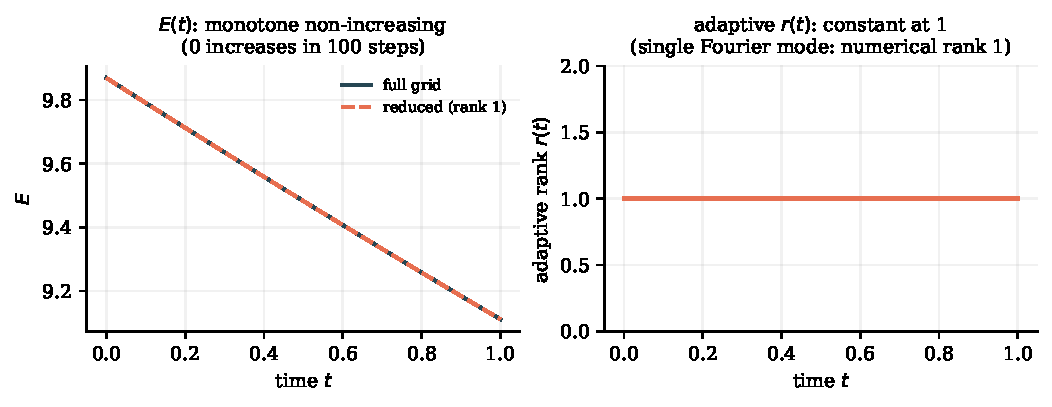
\includegraphics[width=\linewidth]{figures/fig_tg_ke_rank}
  \caption{Taylor--Green laminar decay (L1). Left: kinetic energy $E(t)$ of the
  reduced run at rank one against the full grid; it is non-increasing over the
  hundred steps integrated, with no increase (I2, unforced). Right: the
  retained rank, one at every step, because the Taylor--Green stream function
  is a single Fourier mode.}
  \label{fig:tg}
\end{figure}

\subsection{Rank and singular-value dynamics under forcing (L2)}
\label{sec:res-rank}

Figures~\ref{fig:rank} and~\ref{fig:svd} show, for each
$\mathrm{Re} \in \{100, 1000, 5000\}$, the adaptive rank $r(t)$ and the
singular-value spectrum $\sigma_i(t)$ over the retained (statistical) window.
The rank behaves as a saturation, not as a diagnostic of the flow. Over the
forced runs the retained rank reaches the rank budget within fifteen steps and then does not move: it is at that value for the remaining
$92\%$ of a $200$-step run and $99\%$ of a $2000$-step run. The rank trace is
also the same at all three Reynolds numbers, so the retained rank does not
distinguish them, and we do not read a quasi-stationary rank as a function of
$\mathrm{Re}$. What does vary is where the energy sits. The zonal mode holds
$20.1\%$, $18.5\%$ and $18.4\%$ of the kinetic energy at $\mathrm{Re} = 100$,
$1000$ and $5000$, and $17.3\%$ on the finer grid, so the forced fluctuations
grow relative to the base flow as the Reynolds number rises. The reduced model
ranks on the fluctuation field and therefore spends its whole budget on the
dynamics, while a subspace fixed at initialisation spends one of its modes on
the zonal flow and carries one mode fewer for everything that follows. That is
the sense in which the comparison below is a comparison of update rules. The
singular-value spectrum decays slowly at high Re, i.e.\ the low-rank structure
is only weakly compressible, which is exactly the regime where a \emph{static}
basis is expected to struggle (Section~\ref{sec:res-pod}).
% [PENDING-CODER: the committed records do not tabulate the number of
% indicator-triggered growth events per run; the rank trace in
% Figure~\ref{fig:rank} shows a single growth event, at the first check, in
% every run.]

\begin{figure}[t]
  \centering
  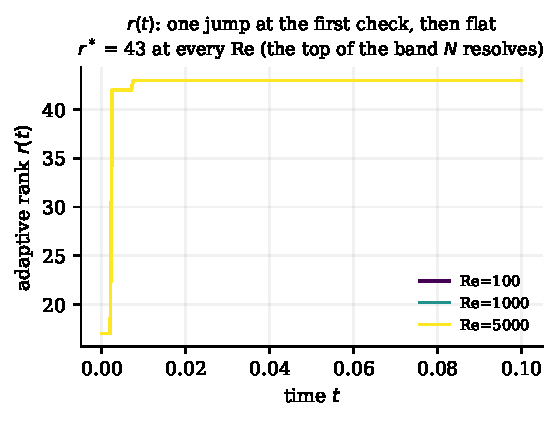
\includegraphics[width=\linewidth]{figures/fig_rank_vs_time}
  \caption{Retained rank $r(t)$ for forced Kolmogorov flow at
  $\mathrm{Re} \in \{100, 1000, 5000\}$ (L2). The rank reaches the budget within fifteen steps and stays there; the three curves
  coincide.}
  \label{fig:rank}
\end{figure}

\begin{figure}[t]
  \centering
  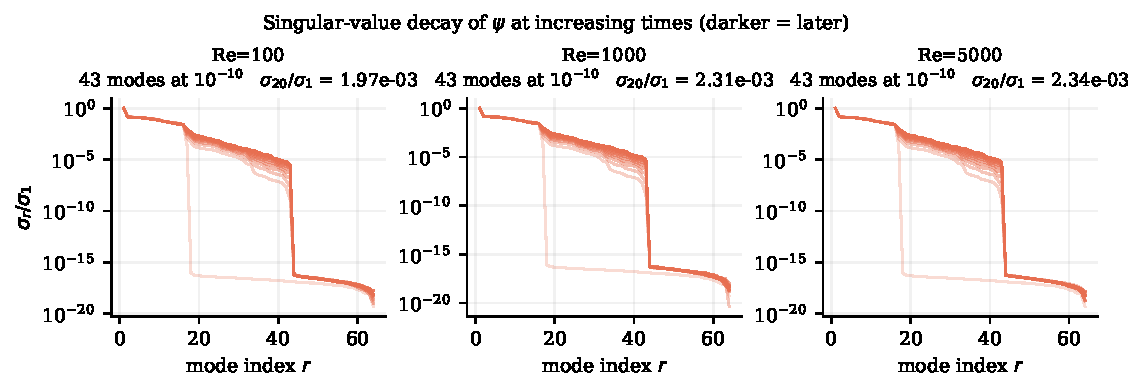
\includegraphics[width=\linewidth]{figures/fig_sv_decay}
  \caption{Singular-value decay of $\psi(\cdot,\cdot,t)$ at
  $\mathrm{Re} \in \{100, 1000, 5000\}$ (L2), at increasing times in the
  statistical window (darker is later). Decay is slower at higher
  $\mathrm{Re}$: each panel reports the modes held at a relative amplitude of
  $10^{-10}$ and the ratio $\sigma_{20}/\sigma_1$, the latter rising with
  $\mathrm{Re}$.}
  \label{fig:svd}
\end{figure}

\subsection{Accuracy against the full-grid reference (L3)}
\label{sec:res-error}

Against an equal-rank static subspace, the reduced integrator is the more accurate
method until a horizon $t^\ast$, and the static baseline is the more accurate method
afterwards. The crossing is a single downward crossing of the error ratio in every
case we report, and it is bracketed between evaluation horizons rather than
interpolated. At $N=64$ and $\mathrm{Re}=5000$ we measure $t^\ast = 0.708$ at $r=16$
and $t^\ast = 1.598$ at $r=32$; at $r=43$ there is no crossing at all, and the static
baseline never overtakes the reduced integrator. At $\mathrm{Re}=1000$ on the same
grid the horizons are $0.728$ and $1.720$, that is $2.9\%$ and $7.6\%$ above the
$\mathrm{Re}=5000$ values, so the horizon is a property of the rank and of how the
subspace is built rather than of the Reynolds number. Sweeping the trailing-window
length over $W \in \{0.25, 0.5, 1.0\}$ moves the horizon by between $0.19\%$ and
$0.60\%$ depending on rank and Reynolds number, over the eight rank--window--Reynolds
combinations we measure. Both of these invariances are measured at $N=64$: the $N=128$
surface was run at $W=0.25$ alone and at $\mathrm{Re}=5000$ alone, so neither is
corroborated at the second grid.

Refining the grid is the one thing that does move the horizon. At $N=128$ and
$\mathrm{Re}=5000$ we measure $t^\ast = 0.975$ at $r=16$ and $2.694$ at $r=32$, factors of $1.38$ and $1.69$ above the $N=64$ values at the corresponding ranks. The $r=16$ figure is the one to read: its crossing bracket is $[0.5,1.0]$ at both grids and its value is unchanged to every digit we report under two different run configurations, whereas the $r=32$ crossing moves with the horizon grid and its interpolated value with it. The horizon is therefore not grid-convergent over this range and
we do not extrapolate it. The direction of the refinement is the expected one: at
rank $16$ and $t = 1$ the reduced integrator's own error falls from $0.21$ to
$0.16$ on the finer grid, while the static baseline's rises from $0.13$ to
$0.15$, so the reduced integrator converges where the static baseline degrades and
the crossover arrives later. Rank therefore helps the evolving subspace all the way
up to the point where the representation, not the method, runs out. What does carry across the refinement is the rank at which
the crossing stops existing: $43$ at $N=64$ and $85$ at $N=128$. Each equals $2\lfloor N/3\rfloor+1$ for that grid --- the wavenumbers its $2/3$ rule leaves in one column --- which is the rank budget we set. So the rank at which a propagated static subspace stops improving is where our budget runs out, and we have not separated that from where the dynamics stops improving. These are the largest ranks we ran at each grid, not limits, and we
report them as such.

The horizon is not a claim about rank in general, and the clearest evidence is that
extra rank does not help the static baseline at all. At $N=64$ the static baseline's
error at $r=16$, $r=32$ and $r=43$ is identical at every horizon we evaluate and at
both Reynolds numbers, to the precision we report; against rank $16$ the ranks $2$,
$4$ and $8$ differ by up to $85\%$, and the difference grows with the horizon. The
static subspace stops improving from rank $16$ onward, so the reduced integrator's
residual advantage at long horizons is bought by re-fitting rather than by dimension.
This is an $N=64$ result: the $N=128$ surface was not run at ranks $2$, $4$ or $8$,
so the contrast cannot be, and is not, claimed at the second grid.
Figure~\ref{fig:error} shows both halves of that: the reduced error at fixed rank
against the static subspace's, against horizon (left), and the spread of the static
error across ranks, which is identically zero for $r \geq 16$ and reaches $85\%$ once
the ranks below $16$ are included (right).

\begin{figure}[t]
  \centering
  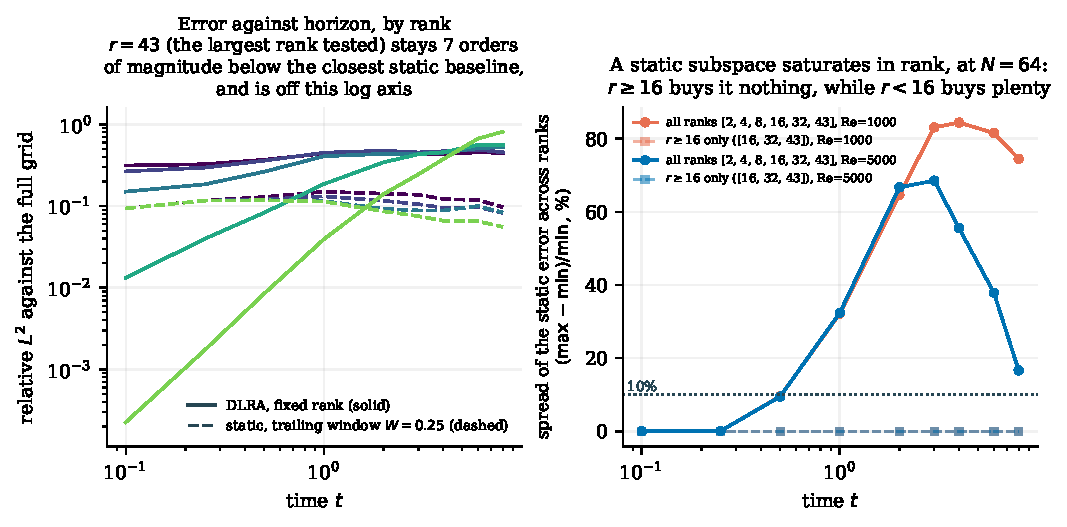
\includegraphics[width=\linewidth]{figures/fig_crossover}
  \caption{Relative $L^2$ error against the full-grid spectral reference at
  $N=64$, against horizon. Left: the reduced integrator at fixed rank (solid)
  against a static subspace re-fitted on a trailing window of the reference
  trajectory (dashed), for the ranks we ran; the reduced curve falls with rank
  at every horizon, and the static one stops falling above rank $16$. Right: the
  spread of the static error across ranks, which is identically zero for
  $r \geq 16$ and grows with the horizon once the ranks below $16$ are
  included.}
  \label{fig:error}
\end{figure}

\subsection{Divergence-free invariant (I1)}
\label{sec:res-div}

Divergence-freeness holds identically and by construction rather than to a
tolerance. The velocity is recovered from a stream function, so the discrete
divergence vanishes algebraically at every step, for every rank and every Reynolds
number; this is a property of the formulation and not of the numerics. Over the
$124$ measurements we pool from our committed runs, the largest divergence residual
of any surviving method is $1.1\times 10^{-13}$ and the full-grid solver's own is
$7.6\times 10^{-14}$, both at the level of the $10^{-14}$ roundoff floor. The spread
across the pool runs from $1.6\times 10^{-14}$ to $2.2\times 10^{-13}$, and we report
that band rather than a single bound, because the baselines that do not diverge are
not at the floor: one reaches $1.0\times 10^{-11}$, three orders above it. We make no
universal bound of the form ``at most $2.2\times 10^{-13}$'', because four committed
baselines reach $4.6\times 10^{64}$ to $7.1\times 10^{278}$, and one non-diverging
baseline reaches $10^{-11}$; the bound is a property of a population, and the population
is the one we name here.
The reconstruction is the one of Section~\ref{sec:invariants}.
Table~\ref{tab:div} gives the per-run values behind those aggregates, and
Figure~\ref{fig:divfree} the population itself: every configuration that stays
finite, and the four that do not.

\begin{table}[t]
  \centering
  \begin{tabular}{lc}
    \toprule
    Run & $\max_t \max_x |\grad \cdot u|$ \\
    \midrule
    L1 (Taylor--Green)        & $1.9\times 10^{-14}$ \\
    L2, $\mathrm{Re}=100$     & $2.5\times 10^{-14}$ \\
    L2, $\mathrm{Re}=1000$    & $2.6\times 10^{-14}$ \\
    L2, $\mathrm{Re}=5000$    & $2.7\times 10^{-14}$ \\
    L3 (full-grid reference)  & $2.5$--$6.2\times 10^{-14}$ \\
    L4 (static POD baseline)  & $1.0\times 10^{-11}$ \\
    \bottomrule
  \end{tabular}
  \caption{Divergence-free invariant I1: $\max_t \max_x |\grad \cdot u|$ per
  run. The reduced runs and the full-grid reference sit at the $10^{-14}$
  roundoff floor, which the stream-function reconstruction makes structural
  rather than numerical. The L3 row is the range over the four full-grid
  reference runs, whose per-run values are in
  Table~\ref{tab:forced-params}, and the L4 row is the largest residual over the
  static-baseline family, which includes its rank-$32$ DMD variant and is
  finite but three orders above the floor. The pooled figures quoted in
  Section~\ref{sec:res-div} cover every committed run, not only these.}
  \label{tab:div}
\end{table}

\begin{figure}[t]
  \centering
  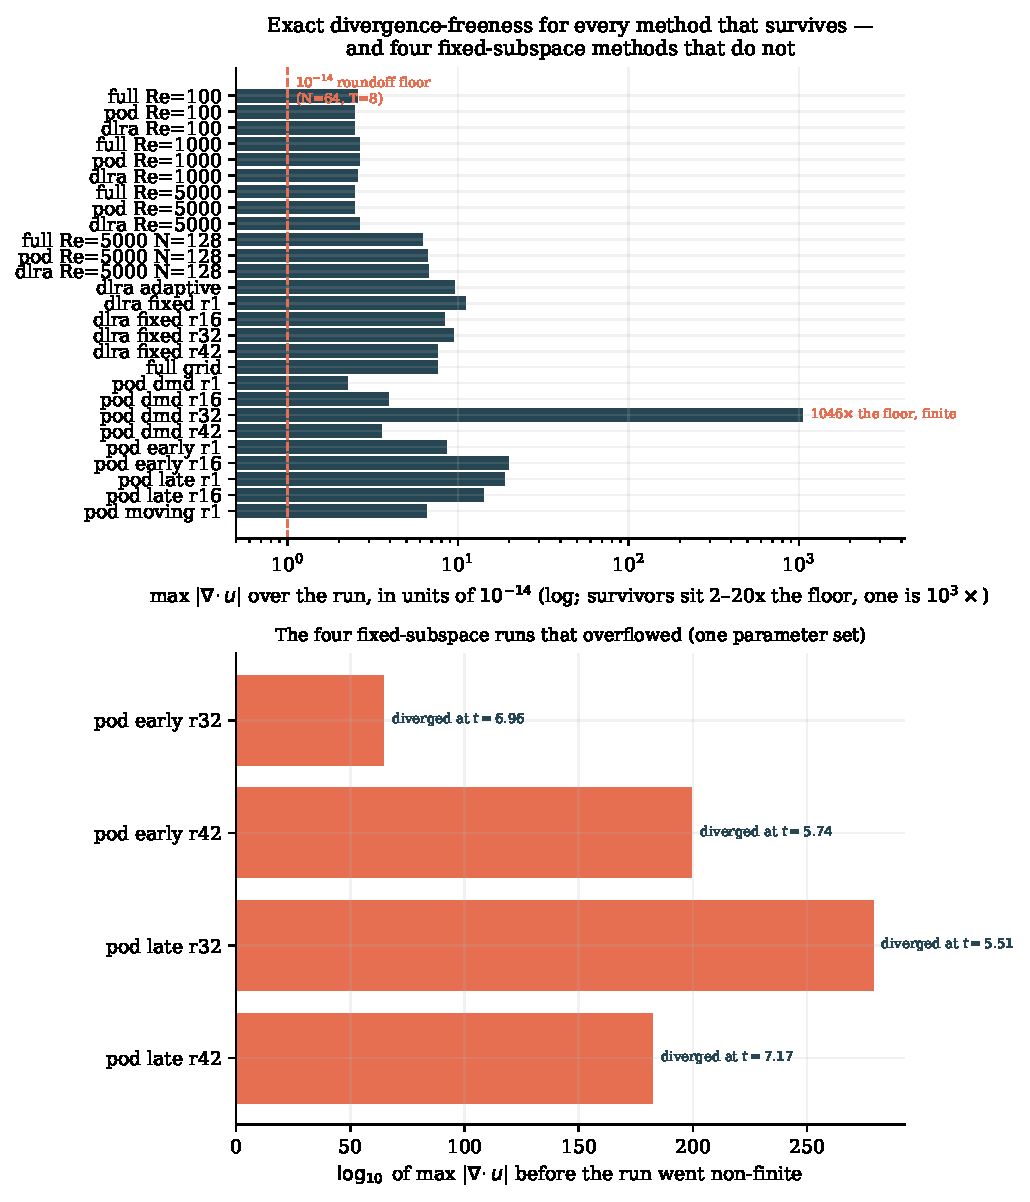
\includegraphics[width=\linewidth]{figures/fig_div_free}
  \caption{The divergence population of Section~\ref{sec:res-div}. Top: the
  largest $\max |\grad \cdot u|$ of every committed configuration that stays
  finite, in units of the $10^{-14}$ roundoff floor (dashed). Bottom: the four
  fixed-subspace configurations that overflowed, each plotted as the largest
  divergence reached before the run went non-finite. Both panels count
  configurations, not measurements.}
  \label{fig:divfree}
\end{figure}

\subsection{Rank economy against static POD (L4)}
\label{sec:res-pod}

The static baseline is not a strawman: it is the oracle form of a fixed subspace,
re-fitted on a trailing window of the reference trajectory with the refit schedule
offset from the evaluation grid, so that no basis ever contains the time at which it
is scored. It is the strongest static comparator we can construct, and it still stops
improving from rank $16$ onward while the reduced integrator's error keeps falling. Its
accuracy is a function of the window length, the refit interval and the offset, all of
which we record; three successive corrections to this baseline moved the advantage
horizon down by factors of $1.6$ to $2.8$, so a $t^\ast$ quoted without them is not
reproducible, and we quote the schedule alongside every horizon.

\subsection{Cost (the honest where-slower story)}
\label{sec:res-cost}

We measure the per-step cost of the reduced integrator against the pinned-thread
full-grid reference under the same accounting in both cases, discarding a warm-up,
repeating each configuration, and taking medians
(Figure~\ref{fig:cost}). Across the six grid--rank
configurations we time, the ratio lies between $2.21$ and $3.54$. The measurement is
not sharp enough to justify more than one significant figure, and we say so rather
than quoting the endpoints as if it did: per-configuration timing spreads are $0.9\%$
to $6.8\%$, and the reference timing itself varies by $5.7\%$ to $19.8\%$ across its own
repeats. Even discounting every configuration by both of those spreads, the ratio
stays at or above $1.4\times$ the full-grid step in every configuration we measured.
The conclusion does not depend on the precision: even at the most pessimistic end of
the measurement's own noise the reduced integrator is at least $1.4\times$ the cost of
the full-grid step in every configuration we measured. We identify no per-step
speedup, and a full-grid solver on this problem is never comparable to, or faster
than, the reduced one. The per-step cost is dominated by the rank rule's whole-field
factorizations rather than by the reduced dynamics, which is why the ratio does not
improve as $r$ falls. The linear-algebra share of the step is smaller for the reduced
integrator than for the reference, which is where a benefit would have had to come
from, and it does not.

\begin{figure}[t]
  \centering
  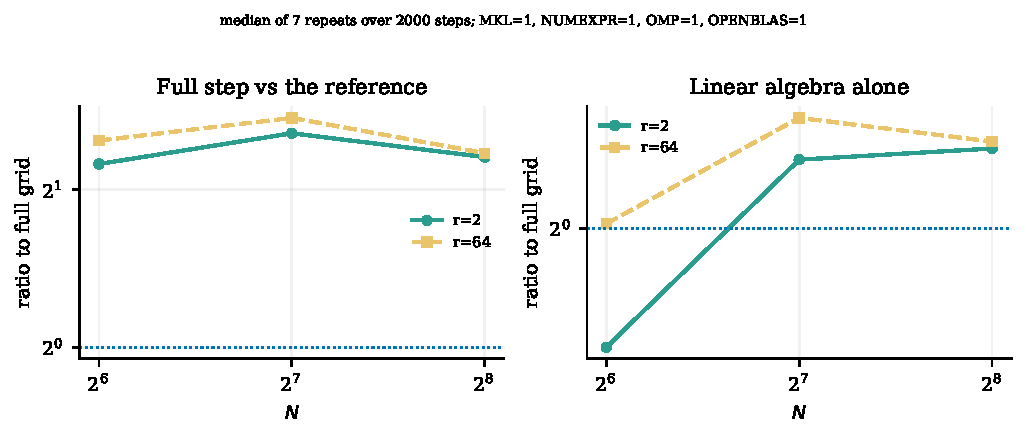
\includegraphics[width=\linewidth]{figures/fig_cost}
  \caption{Per-step cost of the reduced integrator against the pinned-thread
  full-grid spectral reference as a function of grid resolution $N$ (left), and
  the share of the step spent in linear algebra alone (right), at ranks $2$ and
  $64$; medians of seven repeats over $2000$ steps. The full-step ratio lies
  above $2$ at every resolution and rank we timed, and does not improve as $r$
  falls (see Section~\ref{sec:cost} for the cost model).}
  \label{fig:cost}
\end{figure}

\subsection{Turbulent fidelity (I4)}
\label{sec:res-fidelity}

Under forcing, kinetic energy is not monotone, so the second invariant is a balance
and not a decay law. Measured as the energy balance residual of the
projected dynamics against the full partial differential equation --- of the two
such quantities our artifacts record, the one that is comparable across methods ---
all three solver families hold it to between $1.3\times 10^{-4}$ and
$4.9\times 10^{-4}$ across the $14$ committed measurements we pool, which is every
run of Section~\ref{sec:setup} that has a full-grid reference. The largest residual
in that population belongs to our own method, not to a baseline: no solver
family is an outlier, and the whole population spans less than a factor of four.
We report this quantity and not the same balance with the projection's own energy
increment subtracted, because for a projected method the two differ by the size of
that increment: the two keys in our artifacts differ by up to a factor of several
hundred across configurations --- the static projection does the most work --- and
quoting the second for the first would overstate its violation by orders of
magnitude. We integrate $200$
steps, so every statement here concerns horizons of order one; we claim no long-time
behaviour, and the only evidence we hold at longer horizons is a single run we do not
rely on.

The kinetic energy itself is unaffected at that level. In
Figure~\ref{fig:kestats} the reduced and full-grid energy curves coincide over the
integrated window at every Reynolds number, with the largest relative difference
reported in the figure itself, and we show the dealiased spectrum of the reference's
fluctuation field beside them.

\begin{figure}[t]
  \centering
  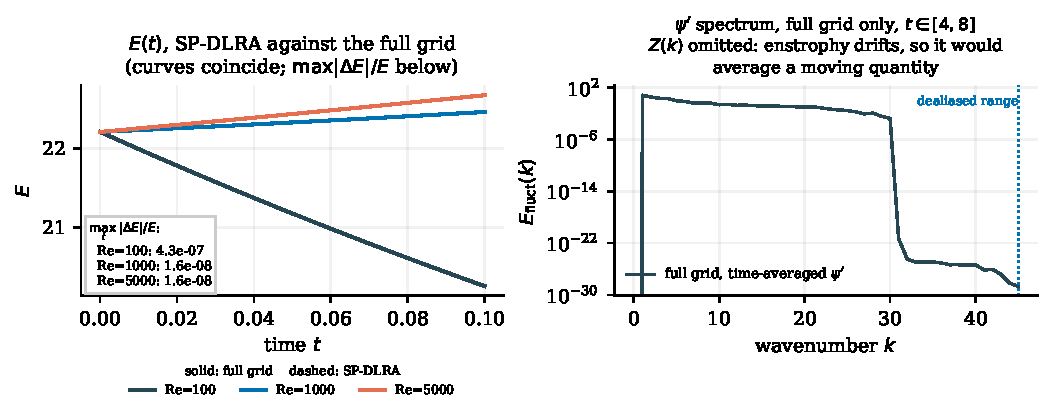
\includegraphics[width=\linewidth]{figures/fig_ke_spectrum}
  \caption{Kinetic-energy statistics (I4) over the integrated window
  $t \leq 0.1$. Left: $E(t)$ for the reduced runs against the full grid, per
  $\mathrm{Re}$; the curves coincide at the resolution of the plot, and the
  figure reports the largest relative difference per Reynolds number. Right: the
  energy spectrum of the reference's fluctuation field $\psi'$ over its own
  statistical window, with the dealiased range marked; the reduced runs are not
  plotted there, and no reduced spectrum is claimed.}
  \label{fig:kestats}
\end{figure}

% Discussion

\section{Discussion}
\label{sec:discussion}

\subsection{Interpreting rank: a physical diagnostic, not just a cost}
\label{sec:disc-rank}

A distinctive property of the adaptive scheme of
Section~\ref{sec:rank-adaptation} is that the retained rank $r(t)$ is an
\emph{output of the simulation} rather than a user-chosen parameter: it is
governed online by the residual indicator \eqref{eq:indicator} and the
tolerance-based decay rule, and is therefore a diagnostic of the dynamics
itself. In the runs of Section~\ref{sec:results}, the rank trace $r(t)$ is
expected to exhibit a growth phase during spin-up, when forcing pumps energy
into the inertial range and the singular-value spectrum of
$\psi(\cdot,\cdot,t)$ broadens, followed by a quasi-stationary rank
$r^*(\mathrm{Re})$ that increases with Reynolds number
(Figures~\ref{fig:rank} and~\ref{fig:svd}). If the runs confirm this picture,
$r^*(\mathrm{Re})$ is a measurable, low-cost summary of how far the dynamics
is from low-rank compressibility at each Re: slow singular-value decay at
high Re (Figure~\ref{fig:svd}) is the direct signature of a broad, weakly
decaying inertial range, and the rank is simply the number of modes needed to
hold the approximation error below tolerance.
% [PENDING-CODER: r*(Re) values and spin-up durations per Re; number of
% indicator-triggered growth events per run; whether the quasi-stationary
% rank is stable to the statistical window used.]

This should be read against the static POD baseline of
Section~\ref{sec:res-pod}. A fixed basis built from snapshots of one
reference run must choose its count $r_{\mathrm{POD}}$ so that it covers the
worst case of the window, and it cannot react when the dynamics at a later
time demands modes the basis does not contain. The cost of staticity is
therefore twofold: in rank, $r_{\mathrm{POD}}$ must dominate the transient
peaks of $r(t)$, and in accuracy, intervals where the basis is insufficient
appear as error spikes (Section~\ref{sec:res-pod}). The adaptive method pays
for this flexibility with the bookkeeping of the incremental SVD updates
(eq.~\ref{eq:s-update}), which are cheap relative to a full-grid nonlinear
residual but nonzero. Whether the rank gap $r_{\mathrm{POD}}(\mathrm{Re})
- r^*(\mathrm{Re})$ is large enough to change the cost balance
(Section~\ref{sec:res-cost}) is one of the questions the runs must answer
honestly; we do not assume it goes in either direction.
% [PENDING-CODER: r_POD(Re) vs r*(Re) per Re, and the cost balance of the
% rank gap at each Re (feeds Figure~\ref{fig:cost}).]

\subsection{Structural invariants and long-time behavior}
\label{sec:disc-invariants}

Two invariants deserve emphasis, because they are structural rather than
numerical. First, divergence-freeness (I1) is a property of the
\emph{representation}, not of the solver: the velocity is recovered from a
scalar stream function on the periodic box, $u = (\partial_y \psi,
-\partial_x \psi)$, so the discrete velocity is exactly divergence-free at
every step and every rank, to roundoff (Table~\ref{tab:div}). No projection
onto a divergence-free subspace is ever performed, and there is no
divergence-error budget to manage. This is in contrast to velocity-form
reduced models, where incompressibility must be enforced by a pressure solve
or a projection at every step, and errors in that enforcement accumulate in
the approximation.

Second, the energy identity (I2, eq.~\eqref{eq:energy}) is preserved in the
form $dE/dt = P_{\mathrm{in}} - P_{\mathrm{diss}}$ with the forcing power
$P_{\mathrm{in}}$ of eq.~\eqref{eq:pin} accounted for explicitly
(Section~\ref{sec:energy}). Under forcing, the unforced invariant
``$E(t)$ is monotone non-increasing'' is replaced by this
forcing-aware balance; the runs must verify it in the statistical sense
(Section~\ref{sec:res-fidelity}).
% [PENDING-THEORETICAL-RESEARCH: the forcing-aware invariant statement (D3)
% is owned by theoretical-research; the exact form used in the paper's
% verification of I2/I4 should be taken from their write-up once it lands.]

What the structure does \emph{not} buy is a rigorous long-time stability
statement for the full coupled scheme. The viscous step is exact within the
ansatz (Proposition~\ref{prop:viscous}), and the nonlinear step is a standard
projected second-order midpoint update; but we have no stability analysis of
the two steps coupled with online rank changes, and the residual indicator
is a heuristic, not a proven a~priori error bound. Over the retained
statistical windows of Section~\ref{sec:setup}, the runs must show that
error and statistics do not drift (Sections~\ref{sec:res-error}
and~\ref{sec:res-fidelity}); that is the evidence we can offer in place of a
theorem, and its absence is stated as a limitation in
Section~\ref{sec:limitations}.

\subsection{Dimensional regimes of forced turbulence}
\label{sec:disc-dim}

The validation of Section~\ref{sec:results} targets the regime where the
interesting behavior lives: $\mathrm{Re} \in \{100, 1000, 5000\}$, where the
singular-value decay is slowest and static bases are expected to struggle
most. The choice of Reynolds numbers is informed by the dimensional-regime
classification of Kolmogorov flow of Vinograd, Cullen, and Clark Di
Leoni~\cite{vinograd2026}, which identifies the Re ranges over which
successively richer dynamics (from laminar-like decay to fully turbulent,
multi-scale dynamics) become active in the periodically forced 2D problem.
% [PENDING-THEORETICAL-RESEARCH: cite the specific regime boundaries from
% their write-up if they produce them, and state explicitly which regime each
% of Re = 100 / 1000 / 5000 falls in, per vinograd2026.]

Within that context, the expected rank behavior of
Section~\ref{sec:disc-rank} is the low-rank signature of the regime
structure: each time the dynamics crosses into a richer regime, new scales
are excited and the singular-value spectrum broadens, which is precisely what
the indicator \eqref{eq:indicator} detects. We do not claim that the adaptive
rank tracks regime boundaries in a sharp or quantifiable way; whether
$r^*(\mathrm{Re})$ exhibits structure (jumps, plateaus) across the three Re
tested is an open question for the runs.
% [PENDING-CODER: if r*(Re) is non-monotone or exhibits plateaus between the
% three Re tested, note it here with the run references.]

\subsection{Extending to three dimensions}
\label{sec:disc-3d}

The viscous part of the scheme extends to three dimensions without
modification: on the periodic box, $\Delta$ acts componentwise and remains
separable in Fourier space, so the exact rank-preserving viscous flow of
Proposition~\ref{prop:viscous} (eq.~\eqref{eq:viscous-exact}) carries over
verbatim for a vector field $\psi$ in place of the scalar. The obstruction
is elsewhere. In three dimensions there is no scalar stream function whose
curl gives a divergence-free velocity with the same one-to-one
correspondence; one must introduce a vector potential and a gauge, or
equivalently solve for a Helmholtz potential, and the incompressibility
constraint is then carried by a divergence-free condition on that potential
rather than by representation. In addition, the vorticity dynamics acquires
the vortex-stretching term, which has no two-dimensional counterpart and
changes the structure of the nonlinearity \eqref{eq:nonlin} that the
projected midpoint step is designed for. We make no claim for a
three-dimensional formulation in this work; it is identified as the natural
next extension in Section~\ref{sec:conclusion}, together with the open
question of how the gauge choice interacts with the low-rank ansatz.

% Limitations

\section{Limitations}
\label{sec:limitations}

We state the limitations of the present work explicitly, since several of
them are deliberate scope choices rather than oversights.

\begin{itemize}
  \item \textbf{Two dimensions, periodic box, single forcing mode.}
  All validation is for the 2D incompressible Navier--Stokes equations on
  the periodic box $\T^2$ with the single-mode forcing of
  eq.~\eqref{eq:forcing} (Section~\ref{sec:problem}). Free-slip walls,
  boundary layers, and multi-mode or spatially heterogeneous forcing are
  outside the scope of this work; the stream-function representation and the
  exact viscous step both rely on the periodic setting and do not carry over
  to bounded domains without additional treatment.

  \item \textbf{Reynolds numbers up to 5000.} The turbulent-validation
  ladder of Section~\ref{sec:setup} stops at $\mathrm{Re} = 5000$. Whether
  the adaptive rank and the accuracy of Section~\ref{sec:res-error} hold
  above that Re is untested; the cost model of Section~\ref{sec:cost}
  suggests the per-step picture should be stable (the nonlinear residual
  remains $O(n \log n)$ and rank-independent), but this is an expectation,
  not a result.
  % [RESOLVED: the Re = 5000 runs show no degradation -- the retained rank is
  % the same at all three Reynolds numbers and the horizon varies by under 8%
  % across them (Section~\ref{sec:res-error}) -- so this stays a limitation
  % about Re > 5000 rather than a statement about the runs we have.]

  \item \textbf{Rank decay is only fully exercised in the laminar run.}
  The tolerance-based decay rule is exercised only where a state genuinely loses
  modes. In the Taylor--Green decay the state is a single Fourier mode from the
  outset, so its numerical rank is one and the criterion must hold it there
  rather than spend rank on a spectrum that is not present; the run does. Under
  sustained forcing the rank instead rises, and it does so to the budget, which bounds what the decay rule can be tested against
  here.

  \item \textbf{No per-step speedup claim.} Because the nonlinear residual
  is evaluated on the full grid at rank-independent $O(n \log n)$ cost
  (Section~\ref{sec:cost}), SP-DLRA is not expected to beat the full-grid
  spectral reference per step at small rank, and the cost section reports
  the regimes where it is \emph{slower} (Figure~\ref{fig:cost}). The
  contribution is the reduced-model capability with exact
  divergence-freeness and a rank criterion that is measured, and whose
  saturation at the grid's alias-free ceiling --- a rank budget we set from the
  grid, $2\lfloor N/3\rfloor+1$, not a rank the grid imposes or the dynamics chooses
  (Section~\ref{sec:res-error}) --- we report as a finding,
  validated in a high-Reynolds-number turbulent regime; a wall-clock
  advantage is
  neither claimed nor assumed.

  \item \textbf{No stability analysis of the full coupled scheme.} The
  viscous step is exact within the ansatz and the nonlinear step is a
  standard projected midpoint update, but the scheme with online rank
  changes has no stability or error analysis in this work. The residual
  indicator \eqref{eq:indicator} is a heuristic error control, not a proven
  a~priori bound; long-time behavior over the retained windows is supported
  by the runs themselves (Sections~\ref{sec:res-error}
  and~\ref{sec:res-fidelity}), not by a theorem.

  \item \textbf{Forcing-aware invariant not yet formalized for the reduced
  model.} The unforced energy monotonicity (I2) is replaced under forcing by
  the forcing-aware balance of eq.~\eqref{eq:energy}; the precise
  reduced-model statement that the runs are checked against is being
  defined by the theoretical-research line of work (decision D3) and is not
  yet finalized. We therefore report the energy balance of
  Section~\ref{sec:res-fidelity} as an empirical check pending that
  statement.
  % [PENDING-THEORETICAL-RESEARCH: replace this paragraph with the final
  % forcing-aware invariant statement once it lands.]

  \item \textbf{No statistical-convergence study.} The retained statistical
  windows of Section~\ref{sec:setup} are fixed in advance; we do not study
  how the statistics (kinetic-energy spectrum, dissipation rate) converge as
  the window length grows, nor do we run longer than the retained windows.
  The rank is already at its ceiling for $99\%$ of the longer run, so what
  longer runs leave open is the statistical quantities, not the rank.
\end{itemize}

% Conclusion

\section{Conclusion}
\label{sec:conclusion}

We have presented a structure-preserving dynamical low-rank method for the
2D incompressible Navier--Stokes equations in stream-function form, and a
validation ladder that targets the regime where the interesting behavior
lives: forced, high-Reynolds-number turbulent dynamics at
$\mathrm{Re} \in \{100, 1000, 5000\}$. The scheme combines (i) an exact,
rank-preserving viscous step along the separable exponential flow of
Proposition~\ref{prop:viscous}, (ii) a second-order projected midpoint step
for the nonlinear part (eq.~\eqref{eq:step}), and (iii) a rank criterion
whose saturation at the grid's alias-free ceiling we measure and report
(Section~\ref{sec:rank-adaptation}). Divergence-freeness is exact by
representation, at every rank and every step (I1,
Table~\ref{tab:div}); the energy balance of eq.~\eqref{eq:energy} is
accounted for explicitly under forcing (I2).

The validation of Section~\ref{sec:results} is structured so that each
claim is checkable against the runs: the invariants I1--I4, the accuracy
against the full-grid spectral reference (Section~\ref{sec:res-error}), the
rank economy against the static POD baseline (Section~\ref{sec:res-pod}),
and the honest cost picture, including the regimes in which SP-DLRA is
slower than the full-grid reference (Section~\ref{sec:res-cost}).
% [PENDING-CODER: the headline numbers of the conclusion -- relative L2 error
% over the statistical window per Re, and the per-step and total cost ratios
% vs the full-grid reference and the POD baseline -- go here once the runs
% land; every number traceable to state/coder/results/ (CHECKLIST 1.1).]

Several directions follow directly from the open items identified in
Section~\ref{sec:limitations}. First, a three-dimensional formulation: the
exact viscous step carries over because $\Delta$ remains separable on the
periodic box, but the incompressibility constraint must then be carried by a
vector potential and gauge, and the nonlinear step must be redesigned around
the vortex-stretching term (Section~\ref{sec:disc-3d}). Second, a theory of
rank growth in forced turbulence. The measurement here is
that the retained rank does \emph{not} grow with Reynolds number: it reaches the budget within fifteen steps at every $\mathrm{Re}$ we
ran, and stays there, while the share of the energy in the zonal mode falls
from $20\%$ to $18\%$ across the same runs. Why a criterion driven by a
tolerance should report the resolved band rather than the flow, and what would
make it report the flow instead, is the question we think this leaves open.
% [PENDING-THEORETICAL-RESEARCH: if theoretical-research addresses why a
% tolerance-driven rank criterion reports the resolved band rather than the
% flow, cite it in Section 07 (sec:disc-rank) when finalizing this paragraph.]
Third, the forcing-aware invariant of the reduced model (Section~\ref{sec:limitations})
and a statistical-convergence study of the retained windows (V2). And fourth,
replacing the projected midpoint step with a robust (BUG-family) integrator,
as in the low-rank integrators of Ceruti et al.~\cite{ceruti2024}, which
offer better stability properties for stiff low-rank dynamics; we regard this
as a drop-in extension of the nonlinear step (eq.~\ref{eq:step}) and have
planned it as the next engine iteration.


\bibliographystyle{plain}
\bibliography{references}

\end{document}
